\documentclass{clbthesis}

\usepackage[utf8]{inputenc}
\usepackage{graphicx}
\usepackage{amsmath}
\usepackage{amsfonts}
\usepackage{listings}
\usepackage{tikz}
\usepackage[square,sort,comma,numbers]{natbib}
\usetikzlibrary{arrows.meta}

\usepackage[T1]{fontenc}


\begin{document}
\catcode`\_=12
\title{Satogaeri}
\mailaddress{csap3977@student.uibk.ac.at}
\matriculationnumber{1117367}
\author{Markus Leitner}
\date{\today}
\supervisor{Univ.-Prof.~Dr.~Aart Middeldorp}
\abstract{%% LaTeX2e file `abstract.tex'
%% generated by the `filecontents' environment
%% from source `CLaTeX' on 2014/11/11.
%%
}
\maketitle 
\tableofcontents


\begin{tikzpicture}
\begin{scope}[scale=1.5]
    \draw[very thick] (0, 0) grid (4, 4);
    
    
	

	
	
\end{scope}
\end{tikzpicture}

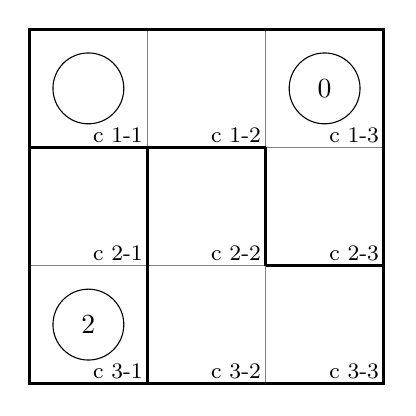
\begin{tikzpicture}
\begin{scope}[scale=1.5]
    \draw[gray] (0, 0) grid (3, 3);
	\draw[very thick, black] (0, 0) rectangle (3, 3);
	\draw[very thick] (0, 2)--(2, 2);
	\draw[very thick] (2, 1)--(3, 1);
	
	\draw[very thick] (1, 0)--(1, 2);
	\draw[very thick] (2, 1)--(2, 2);
	
	\draw (0.5, 2.5) circle [radius=0.3];
	\node[anchor=center] at (2.5, 2.5) {0};
	\draw (2.5, 2.5) circle [radius=0.3];
	\node[anchor=center] at (0.5, 0.5) {2};
	\draw (0.5, 0.5) circle [radius=0.3];
	\node[anchor=center, font=\footnotesize] at (0.75, 2.1) {c 1-1};
	\node[anchor=center, font=\footnotesize] at (1.75, 2.1) {c 1-2};
	\node[anchor=center, font=\footnotesize] at (2.75, 2.1) {c 1-3};
	\node[anchor=center, font=\footnotesize] at (0.75, 1.1) {c 2-1};
	\node[anchor=center, font=\footnotesize] at (1.75, 1.1) {c 2-2};
	\node[anchor=center, font=\footnotesize] at (2.75, 1.1) {c 2-3};
	\node[anchor=center, font=\footnotesize] at (0.75, 0.1) {c 3-1};
	\node[anchor=center, font=\footnotesize] at (1.75, 0.1) {c 3-2};
	\node[anchor=center, font=\footnotesize] at (2.75, 0.1) {c 3-3};
	
\end{scope}
\end{tikzpicture}

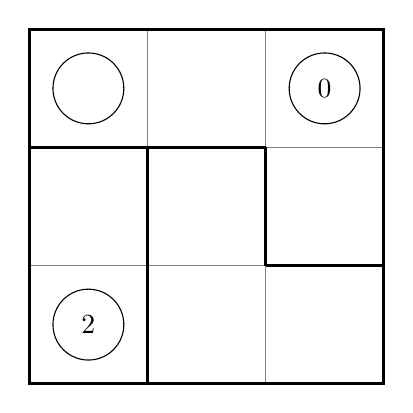
\begin{tikzpicture}
\begin{scope}[scale=1.5]
    \draw[gray] (0, 0) grid (3, 3);
	\draw[very thick, black] (0, 0) rectangle (3, 3);
	\draw[very thick] (0, 2)--(2, 2);
	\draw[very thick] (2, 1)--(3, 1);
	
	\draw[very thick] (1, 0)--(1, 2);
	\draw[very thick] (2, 1)--(2, 2);
	
	\draw (0.5, 2.5) circle [radius=0.3];
	\node[anchor=center] at (2.5, 2.5) {0};
	\draw (2.5, 2.5) circle [radius=0.3];
	\node[anchor=center] at (0.5, 0.5) {2};
	\draw (0.5, 0.5) circle [radius=0.3];
	
	
\end{scope}
\end{tikzpicture}

\end{document}
